\documentclass{standalone}

\usepackage{tikz}
\usepackage{standalone}
\usetikzlibrary{calc}
\usepackage{pgfplots}

\begin{document}

    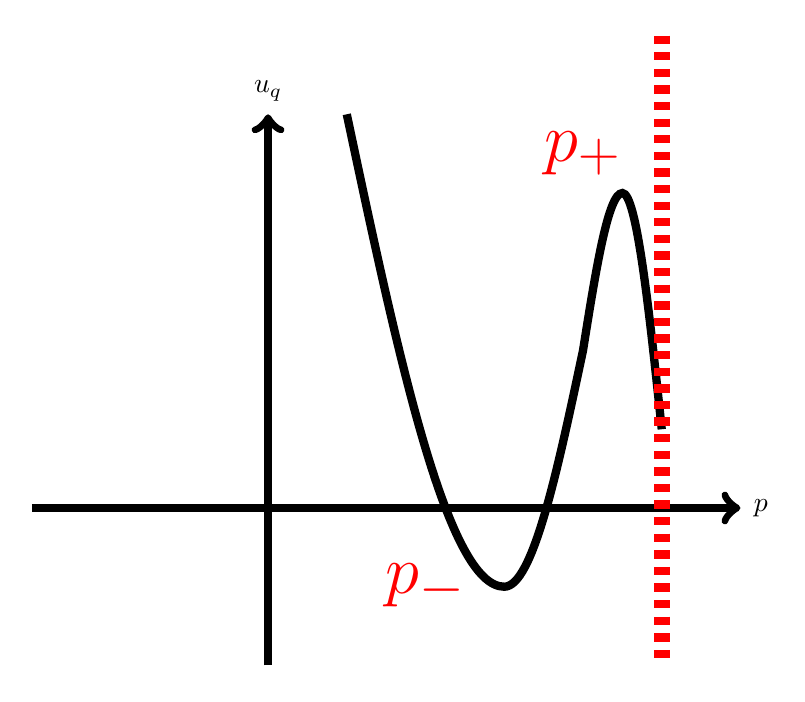
\begin{tikzpicture}

    \draw[->, line width=3pt] (-3, 0) -- (6, 0) node[right] {$p$};
    \draw[->, line width=3pt] (0,-2) -- (0,5) node[above] {$u_q$};

    \draw[line width=3pt] (1, 5) sin (3 , -1) cos (4, 2) sin (4.5, 4) cos (5, 1);

    \node (0) at (2, -1) {\Huge{\textcolor{red}{\(p_{-}\)}}};
    \node (0) at (4, 4.5) {\Huge{\textcolor{red}{\(p_{+}\)}}};

	\draw [dashed, line width=2mm, red] (5,6) -- (5,-2);

    \end{tikzpicture}

\end{document}